
\appendix
\chapter{Extra Masks}

We include some extra masks from our final model taken from all 7 test CT scans.

\begin{figure}[H]
\centering
\label{final_model}
\begin{minipage}{0.45\textwidth}
\centering
{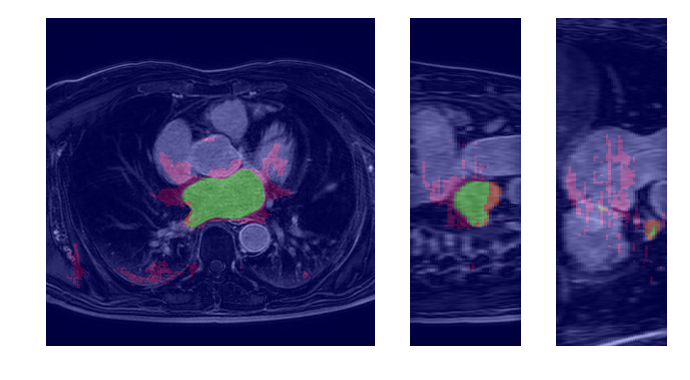
\includegraphics[trim=0cm 2cm 0cm 2cm, clip=true, height=50mm, width=75mm]{Appendix/img/Masks_for_14012303_0.png}}
\end{minipage}\hfill
\begin{minipage}{0.45\textwidth}
\centering
{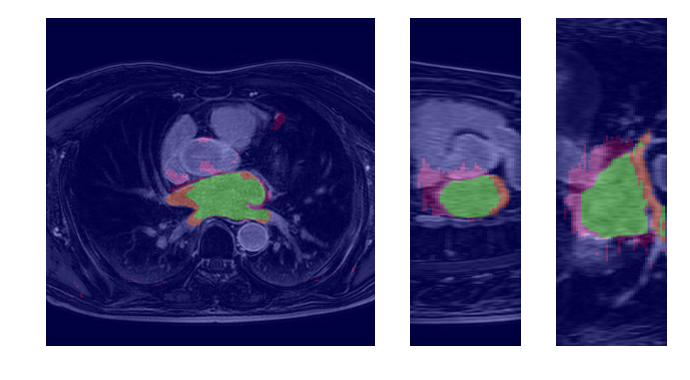
\includegraphics[trim=0cm 2cm 0cm 2cm, clip=true, height=50mm, width=75mm]{Appendix/img/Masks_for_14012303_1.png}}
\end{minipage}
\caption{Two sets of masks taken from CT scan 14012303}
\end{figure}

\begin{figure}[H]
\centering
\label{final_model}
\begin{minipage}{0.45\textwidth}
\centering
{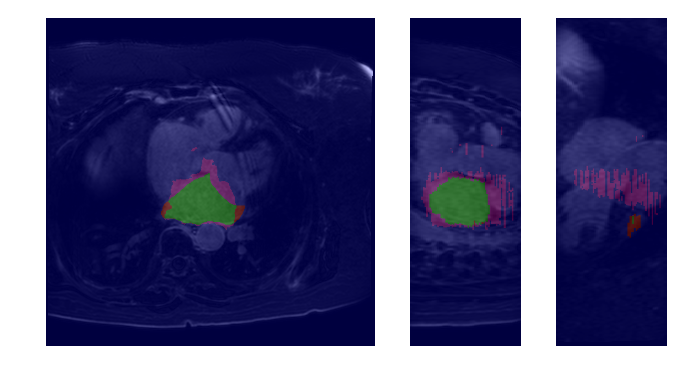
\includegraphics[trim=0cm 2cm 0cm 2cm, clip=true, height=50mm, width=75mm]{Appendix/img/Masks_for_14022801_0.png}}
\end{minipage}\hfill
\begin{minipage}{0.45\textwidth}
\centering
{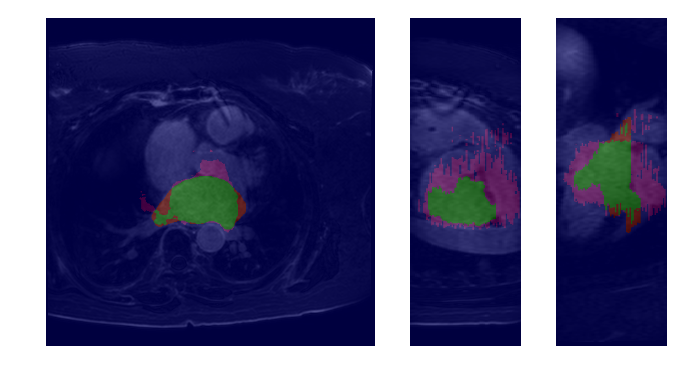
\includegraphics[trim=0cm 2cm 0cm 2cm, clip=true, height=50mm, width=75mm]{Appendix/img/Masks_for_14022801_1.png}}
\end{minipage}
\caption{Two sets of masks taken from CT scan 14022801}
\end{figure}

\begin{figure}[H]
\centering
\label{final_model}
\begin{minipage}{0.45\textwidth}
\centering
{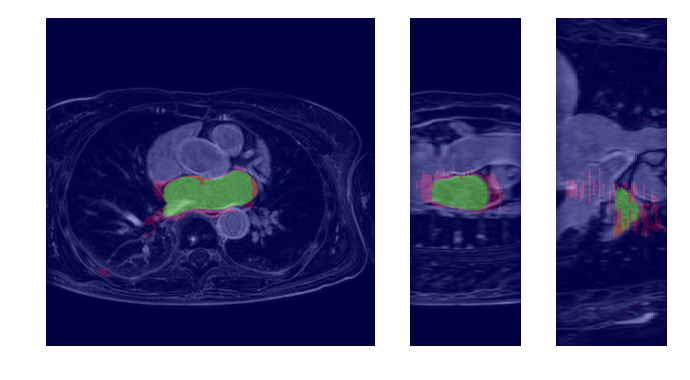
\includegraphics[trim=0cm 2cm 0cm 2cm, clip=true, height=50mm, width=75mm]{Appendix/img/Masks_for_14031001_0.png}}
\end{minipage}\hfill
\begin{minipage}{0.45\textwidth}
\centering
{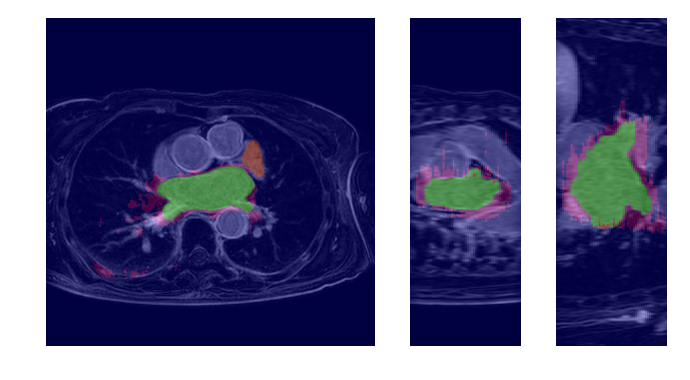
\includegraphics[trim=0cm 2cm 0cm 2cm, clip=true, height=50mm, width=75mm]{Appendix/img/Masks_for_14031001_1.png}}
\end{minipage}
\caption{Two sets of masks taken from CT scan 14031001}
\end{figure}

\begin{figure}[H]
\centering
\label{final_model}
\begin{minipage}{0.45\textwidth}
\centering
{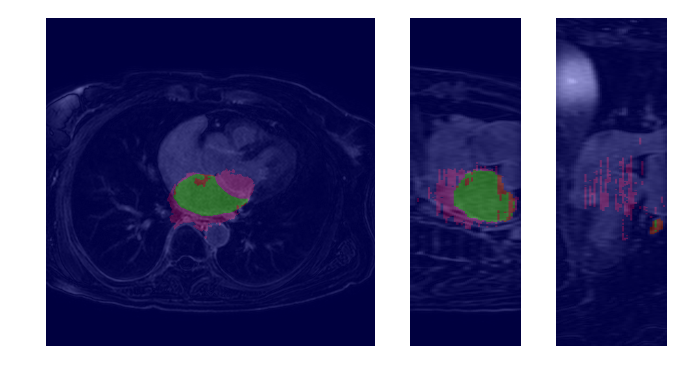
\includegraphics[trim=0cm 2cm 0cm 2cm, clip=true, height=50mm, width=75mm]{Appendix/img/Masks_for_14031201_0.png}}
\end{minipage}\hfill
\begin{minipage}{0.45\textwidth}
\centering
{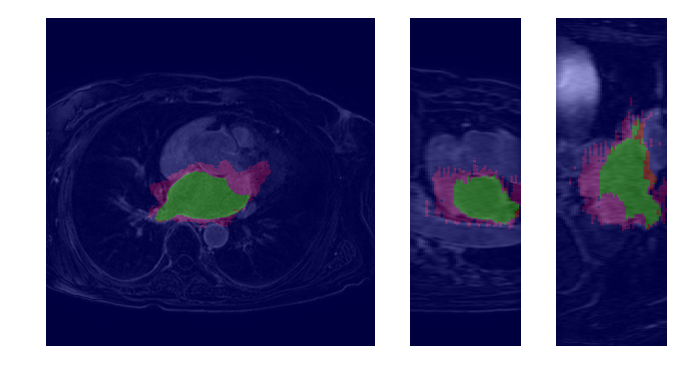
\includegraphics[trim=0cm 2cm 0cm 2cm, clip=true, height=50mm, width=75mm]{Appendix/img/Masks_for_14031201_1.png}}
\end{minipage}
\caption{Two sets of masks taken from CT scan 14031201}
\end{figure}

\begin{figure}[H]
\centering
\label{final_model}
\begin{minipage}{0.45\textwidth}
\centering
{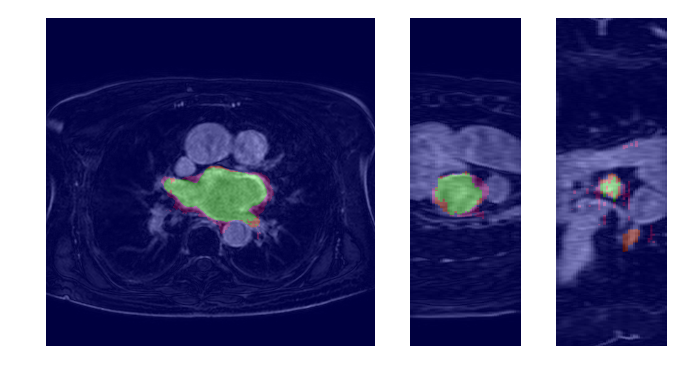
\includegraphics[trim=0cm 2cm 0cm 2cm, clip=true, height=50mm, width=75mm]{Appendix/img/Masks_for_14040204_0.png}}
\end{minipage}\hfill
\begin{minipage}{0.45\textwidth}
\centering
{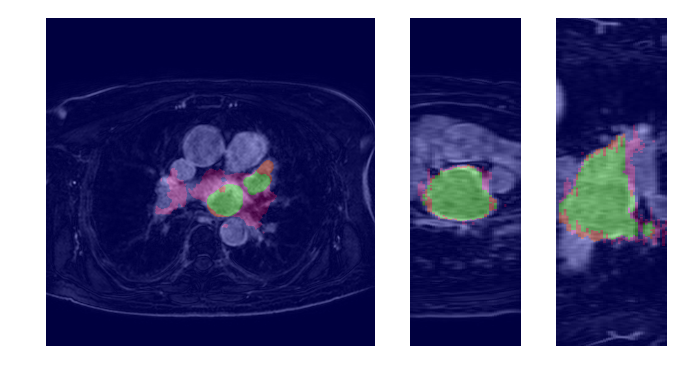
\includegraphics[trim=0cm 2cm 0cm 2cm, clip=true, height=50mm, width=75mm]{Appendix/img/Masks_for_14040204_1.png}}
\end{minipage}
\caption{Two sets of masks taken from CT scan 14040204}
\end{figure}

\begin{figure}[H]
\centering
\label{final_model}
\begin{minipage}{0.45\textwidth}
\centering
{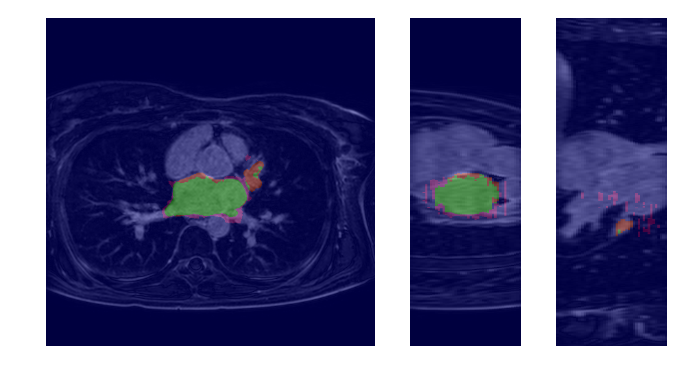
\includegraphics[trim=0cm 2cm 0cm 2cm, clip=true, height=50mm, width=75mm]{Appendix/img/Masks_for_14051403_0.png}}
\end{minipage}\hfill
\begin{minipage}{0.45\textwidth}
\centering
{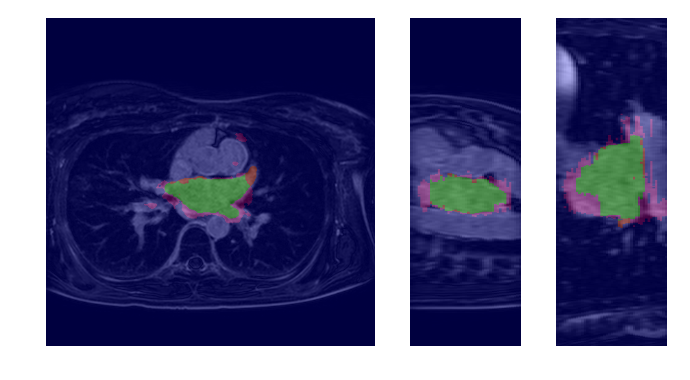
\includegraphics[trim=0cm 2cm 0cm 2cm, clip=true, height=50mm, width=75mm]{Appendix/img/Masks_for_14051403_1.png}}
\end{minipage}
\caption{Two sets of masks taken from CT scan 14051403}
\end{figure}

\begin{figure}[H]
\centering
\label{final_model}
\begin{minipage}{0.45\textwidth}
\centering
{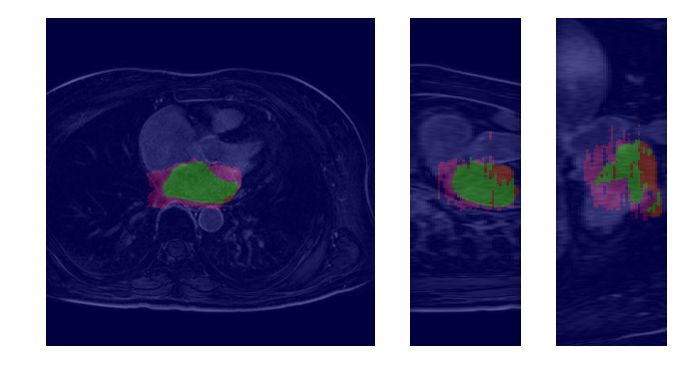
\includegraphics[trim=0cm 2cm 0cm 2cm, clip=true, height=50mm, width=75mm]{Appendix/img/Masks_for_14051404_0.png}}
\end{minipage}\hfill
\begin{minipage}{0.45\textwidth}
\centering
{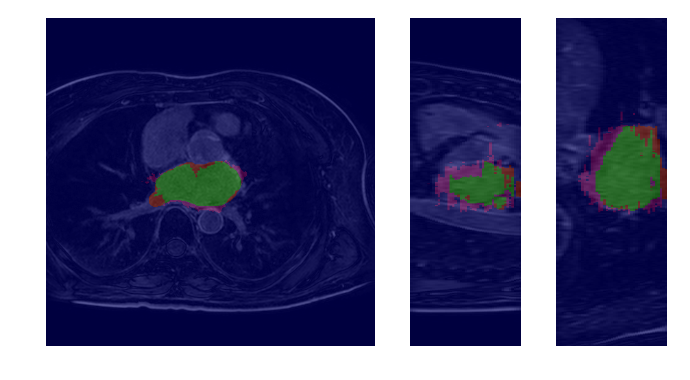
\includegraphics[trim=0cm 2cm 0cm 2cm, clip=true, height=50mm, width=75mm]{Appendix/img/Masks_for_14051404_1.png}}
\end{minipage}
\caption{Two sets of masks taken from CT scan 14051404}
\end{figure}

\chapter{Code}

\lstset{style=myLuastyle}

Only the two most important part of the code for training neural networks are shown: the model and the training function. In the interest of brevity, we omit the rest which deals with handling logistics, data generation and plotting. However, the entire code base can be found on Github at \url{https://github.com/eisenhower444/Master_project}.\\

\noindent The following code defines a model using the nn package in Torch.\\

\begin{lstlisting}
require "nn"
require "cudnn"

----------------------------------------------------------------------
-- Model parameters

-- hidden units, filter sizes:
nfeaturemaps  = { 32, 64, 100 }
filtsize 	  = 5
poolsize 	  = { 2, 2 }
featuremaps_h = 5
featuremaps_w = 5
noutputs 	  = 2

----------------------------------------------------------------------
model = nn.Sequential()

-- stage 1 : mean suppresion -> filter bank -> squashing -> max pooling
model:add(cudnn.SpatialConvolution(nfeats, nfeaturemaps[1], filtsize, filtsize))
model:add(cudnn.ReLU(true))
model:add(cudnn.SpatialMaxPooling(poolsize[1],poolsize[1],poolsize[1],poolsize[1]))
-- stage 2 : mean suppresion -> filter bank -> squashing -> max pooling
model:add(cudnn.SpatialConvolution(nfeaturemaps[1], nfeaturemaps[2], filtsize, filtsize))
model:add(cudnn.ReLU(true))
model:add(cudnn.SpatialMaxPooling(poolsize[2],poolsize[2],poolsize[2],poolsize[2]))
-- stage 2 : standard 1-layer MLP:
model:add(nn.View(nfeaturemaps[2]*featuremaps_h*featuremaps_w))
model:add(nn.Dropout(0.5))
model:add(nn.Linear(nfeaturemaps[2]*featuremaps_h*featuremaps_w, nfeaturemaps[3]))
model:add(nn.ReLU())
model:add(nn.Dropout(0.5))
model:add(nn.Linear(nfeaturemaps[3], noutputs))
model:add(nn.LogSoftMax())

----------------------------------------------------------------------
criterion = nn.ClassNLLCriterion()
\end{lstlisting}

\newpage 

\noindent The following code is the main workhorse for training a neural network on one or many GPUs in Torch.\\

\begin{lstlisting}
-- Multi-GPU set up
if opt.number_of_GPUs > 1 then
    print('Using data parallel')
    local GPU_network = nn.DataParallel(1):cuda()
    for i = 1, opt.number_of_GPUs do
        local current_GPU = math.fmod(opt.GPU_id + (i-1)-1, cutorch.getDeviceCount())+1
        cutorch.setDevice(current_GPU)
        GPU_network:add(model:clone():cuda(), current_GPU)
    end
    cutorch.setDevice(opt.GPU_id)

    model = GPU_network
end

model:cuda()
criterion:cuda()

-- Optimizer
optimator = nn.Optim(model, optimState)

-- Retrieve parameters and gradients:
-- this extracts and flattens all the trainable parameters of the model
if opt.number_of_GPUs > 1 then
    parameters, gradParameters = model:get(1):getParameters()
    cutorch.synchronize()
    model:cuda()  -- get it back on the right GPUs
else
    parameters, gradParameters = model:getParameters()
end

function train()

    -- epoch tracker
    epoch = epoch or 1

    -- set model to training mode (for modules that differ in training and testing, like Dropout)
    model:training()

    -- shuffle at each epoch
    shuffle = torch.randperm(trainData.size())

    -- do one epoch
    for t = 1,trainingSize,opt.batchSize do
        -- disp progress
        xlua.progress(math.min(t+opt.batchSize-1,trainingSize), trainingSize)

        -- create mini batch
	if t < (trainingSize - opt.batchSize) then
		batchSize = opt.batchSize
	else
		batchSize = trainingSize - t - math.fmod((trainingSize - t),opt.number_of_GPUs)
	end

        inputs = torch.Tensor(batchSize,nfeats,patchsize,patchsize)
        targets = torch.Tensor(batchSize)
        for i = t,math.min(t+opt.batchSize-1,trainingSize) do
            -- load new sample
            inputs[{{i%batchSize + 1},{},{},{}}] = trainData.data[shuffle[i]]:clone()
            targets[i%batchSize + 1]             = trainData.labels[shuffle[i]]
        end

        inputs    = inputs:cuda() 
        targets   = targets:cuda()
 	
        f, outputs = optimator:optimize(optim.sgd, inputs, targets, criterion)

        if opt.number_of_GPUs > 1 then cutorch.synchronize() end
    end

    -- next epoch
    collectgarbage()
    epoch = epoch + 1
end
\end{lstlisting}